\documentclass[12pt]{article}
\usepackage{graphicx}
\usepackage[none]{hyphenat}
\usepackage{graphicx}
\usepackage{listings}
\usepackage[english]{babel}
\usepackage{graphicx}
\usepackage{caption} 
\usepackage{booktabs}
\usepackage{gensymb}
\usepackage{array}
\usepackage{amssymb} % for \because
\usepackage{amsmath}   % for having text in math mode
\usepackage{extarrows} % for Row operations arrows
\usepackage{listings}
\lstset{
  frame=single,
  breaklines=true
}
\usepackage{hyperref}
  
%Following 2 lines were added to remove the blank page at the beginning
\usepackage{atbegshi}% http://ctan.org/pkg/atbegshi
\AtBeginDocument{\AtBeginShipoutNext{\AtBeginShipoutDiscard}}


%New macro definitions
\newcommand{\mydet}[1]{\ensuremath{\begin{vmatrix}#1\end{vmatrix}}}
\providecommand{\brak}[1]{\ensuremath{\left(#1\right)}}
\providecommand{\norm}[1]{\left\lVert#1\right\rVert}
\newcommand{\solution}{\noindent \textbf{Solution: }}
\newcommand{\myvec}[1]{\ensuremath{\begin{pmatrix}#1\end{pmatrix}}}
\providecommand{\abs}[1]{\left\vert#1\right\vert}
\let\vec\mathbf

\begin{document}

\begin{center}
\title{\textbf{Equation  of circle}}
\date{\vspace{-5ex}} %Not to print date automatically
\maketitle
\end{center}
\setcounter{page}{1}
\section*{Excercise 10.4}
\begin{enumerate}
\item If two equal chords of a circle intersect within the circle, prove that the segments of one chord are equal to corresponding segments of other chord.
\\
\solution
\\
Consider the Circle of radius $1$ and length of chord be $1.5$
\begin{align}
\vec{c}=\myvec{0\\0},d=1.5,r=1
\end{align}
Consider the points on the circle
\begin{align}
	\vec{P}&=\myvec{\cos\theta_1\\\sin\theta_1}\\
	\vec{Q}&=\myvec{\cos\theta_2\\\sin\theta_2}\\
	\vec{R}&=\myvec{\cos\theta_3\\\sin\theta_3}\\
	\vec{S}&=\myvec{\cos\theta_4\\\sin\theta_4}
\end{align}
So, here
\begin{align}
	(\vec{P}-\vec{Q})&=\myvec{\cos\theta_1-\cos\theta_2\\sin\theta_1-\sin\theta_2}
	\end{align}
	\begin{align}
	\norm{\vec{P}-\vec{Q}}^2&=d^2
		\end{align}
		\begin{align*}
	&\implies\myvec{(\cos\theta_1-\cos\theta_2)^2}+\myvec{(\sin\theta_1-\sin\theta_2)^2}=d^2\\
	&\implies2-2\myvec{\cos(\theta_1-\theta_2)}=d^2\\
	&\implies2(2\myvec{\sin^2(\frac{\theta_1-\theta_2}{2})}=d^2\\
	&\implies\myvec{\sin^2\frac{\theta_1-\theta_2}{2}}=\frac{d^2}{4}\\
	&\implies\myvec{\sin\frac{\theta_1-\theta_2}{2}}=\frac{d}{2}\\
&\implies\myvec{\frac{\theta_1-\theta_2}{2}}=\myvec{\sin^{-1}(0.75)}\\
	\end{align*}
\begin{align}
	\myvec{\theta_1-\theta_2}=97.1806 
	\end{align}
Simillary we can say that
\begin{align}
	\myvec{\theta_3-\theta_4}=97.1806   		       
\end{align}	
Let
\begin{align}
\theta_1=30\degree,\theta_3=60\degree
\end{align}
here
\begin{align}
\vec{P}&=\myvec{\frac{\sqrt{3}}{2}\\[2pt]\frac{1}{2}}\\
\vec{Q}&=\myvec{0.3878\\-0.9217}\\
\vec{R}&=\myvec{\frac{1}{2}\\[2pt]\frac{\sqrt{3}}{2}}\\
\vec{S}&=\myvec{0.7967\\-0.6043}
\end{align}
Obtain the point of intersection of line $\vec{PQ}$,$\vec{RS}$
\begin{align}
\vec{n_1^\top\myvec{\vec{X}-\vec{P}}}&=0\label{15}\\
\vec{n_2^\top\myvec{\vec{X}-\vec{R}}}&=0\label{16}\\
\vec{n_1}&=\myvec{1.4217\\-0.47822}\\
\vec{n_2}&=\myvec{1.4703\\0.2967}
\end{align}
From the Result of python code , we got the point of intersection of \eqref{15} \eqref{16}  is given as :
\begin{align}
\vec{T}&=\myvec{0.68341409\\-0.04288508}
\end{align}
From the Result of python code , we get
\begin{align}
\norm{\vec{P}-\vec{T}}&=0.5727\\
\norm{\vec{R}-\vec{T}}&=0.9272\\
\norm{\vec{Q}-\vec{T}}&=0.9272\\
\norm{\vec{S}-\vec{T}}&=0.5727
\end{align}
Hence, we proved that
\begin{align}
\norm{\vec{P}-\vec{T}}=\norm{\vec{S}-\vec{T}}\\
\norm{\vec{Q}-\vec{T}}=\norm{\vec{R}-\vec{T}}
\end{align} 
\begin{figure}[!h]
	\begin{center} 
	  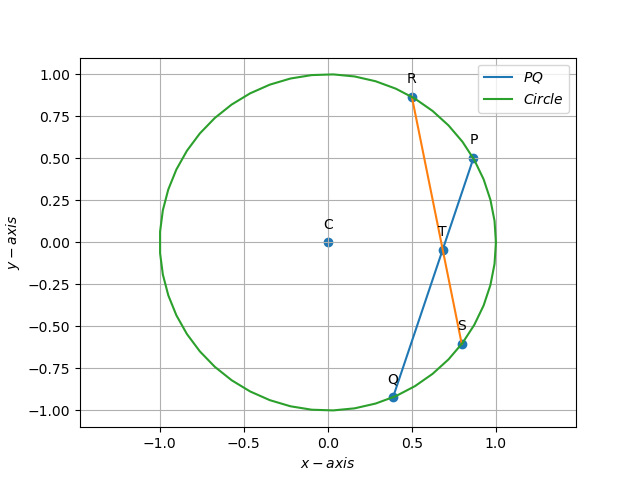
\includegraphics[width=\columnwidth]{/home/srikanth/circle/9.10.4.2/figs/c.png}
	\end{center}
\caption{}
\label{fig:Fig1}
\end{figure}
\end{enumerate}
\end{document}
